\vspace{-13pt}
\section{Basic Idea}
\vspace{-5pt}
\subsection{Fallacy: LBA-based lifetime prediction}
%\vspace{-5pt}
Many existing data separation techniques such as~\cite{AutoStream, HotCold} 
estimate the data lifetime based on the update frequency of LBAs.  
For example, AutoStream~\cite{AutoStream} assumes that, if
some LBAs are frequently rewritten by applications, those LBAs hold hot data.
This LBA-based lifetime prediction 
approach, however, does not work well with recent data-intensive 
applications where a majority of
new data are written in an append-only manner.  



In order to illustrate a mismatch between an LBA-based predictor and 
append-only workloads, we analyzed the write pattern of 
RocksDB~\cite{RocksDB}, which is a
popular key-value store based on the LSM-tree algorithm~\cite{LSM}.
Fig.~\ref{fig:lba_lifetime}(a) shows how LBAs may be related 
to data lifetimes\footnote{The lifetime of data is defined to be 
the number of write requests between when the data is first written 
and when the data is invalidated by an overwrite or a TRIM command.}
in RocksDB~\cite{RocksDB}.  
As shown in Fig.~\ref{fig:lba_lifetime}(a), 
there exists no strong correlation between the LBAs and lifetimes in RocksDB.  
This scatter plot is in sharp contrast with one for update workloads 
where a few distinct LBA regions have short lifetimes while others 
have very long lifetimes.

We also analyzed 
if the lifetimes of LBAs change under some predictable patterns over times 
although the overall lifetime distribution shows large variances.
Fig.~\ref{fig:lba_lifetime}(b) shows a scatter plot of data lifetimes over the logical time 
for a specific 1-MB chunk with 256 pages. 
As shown in Fig.~\ref{fig:lba_lifetime}(b), 
for the given chuck, data lifetimes vary in a random fashion
(although some temporal locality is observed).
\begin{comment}
Over the logical time, the lifetime of data written to the chunk 
varies in an unpredictable fashion.  
For example, at the logical time 10, the lifetime was 1 but it increases about 
2.6 million around the logical time 450 
followed by a rapid drop around the logical time 600. 
\end{comment}
Our illustration using RocksDB strongly suggests that under append-only
workloads, LBAs are not useful in deciding data lifetimes.

\vspace{-10pt}
\subsection{Program context as a lifetime predictor}
%\vspace{-5pt}
In developing \textsf{\small PCStream}, our key insight was that in most applications 
(regardless of their I/O workload characteristics), 
a few dominant I/O activities exist for an application
and each dominant I/O activity   
represents the application's important I/O context (e.g., for logging or for flushing). 
Furthermore, most dominant I/O activities tend to have distinct data lifetime patterns.
In order to distinguish data by their lifetimes, therefore, 
it is important to effectively distinguish dominant I/O activities from each other.  
For example, in update workloads, 
LBAs alone were effective in separating dominant I/O activities.  

\begin{figure}[t]
	\centering
	\vspace{-7pt}
	\subfloat[Lifetime patterns over LBAs]{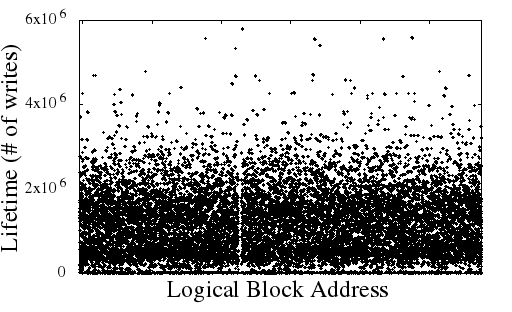
\includegraphics[width=0.25\textwidth]{figure/lba_lifetime2}}  % data from 0/03031641
	\subfloat[Lifetime patterns over time]{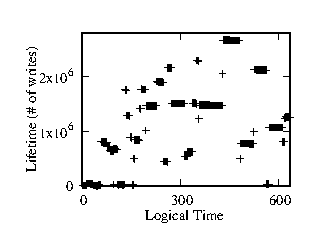
\includegraphics[width=0.22\textwidth]{figure/lifetime_in_chunk2}}
	%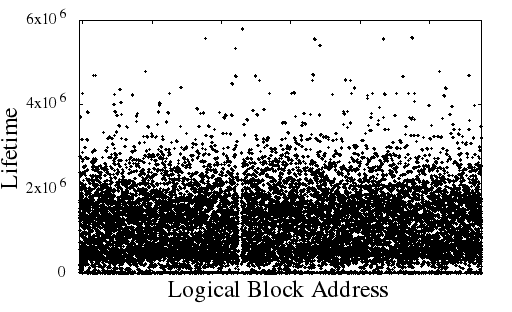
\includegraphics[width=0.9\linewidth]{figure/lba_lifetime} 
	%\vspace{-10pt}
	\vspace{-10pt}
	\caption{Lifetime distributions over addresses and times.} %shane part
		\label{fig:lba_lifetime}
	\vspace{-17pt}
\end{figure}

\begin{comment}
In developing PCStream, we started from a simple question: 
how can we extract I/O context from an application? 
For example, in RocksDB, logging, flushing and compaction can be regarded
as different I/O contexts.
RocksDB appends write-ahead logs to storage to ensure data
persistence.  Those logs have short lifetimes because they are quickly deleted
after original data are persistently stored.
The flush module (which materializes the content of a memtable in
DRAM, called an L0 table, to an L1 table in the storage) generates data
with relatively short lifetimes. This is because an L1 table will be flushed to
an L2 table and be removed in the near future. Conversely, a compaction module
writes long-lived data that are unlikely to be removed for a long time.

The above observation implies that, if we are able to know the detailed
behaviors of append-only applications, data with different lifetimes can be
isolated in separate streams in an SSD. As mentioned before, a common
solution~\cite{MultiStream} to realizing this is manually modify an application
code so that each module assigns a unique stream ID to data it generates.
However, owing to considerable implementation efforts required to modify
individual applications, this approach is not widely used in practice.
\end{comment}

In this paper, we argue that a program context is an efficient  general-purpose
indicator for separating dominant I/O activities regardless of the type of I/O
workloads.  Since a PC represents an execution path of an application which
invokes write-related system functions such as {\tt write()} and {\tt writev()}
in the Linux kernel,  we represent the PC by summing program counter values of
all the functions along the execution path which leads to a write system call.
In RocksDB, for example, dominant I/O activities include logging, flushing and
compaction.  Since they are invoked through different function-call paths, we
can easily identify dominant I/O activities of RocksDB using PCs.  For example,
Fig.~\ref{fig:getpc}(a) shows an execution path for flushing in RocksDB.  The
sum of program counter values of \texttt{Run()}, \texttt{WriteLevel0Table()},
and \texttt{BuildTable()} is used to represent the PC for the flushing
activity.  Note that using the program context to distinguish data lifetimes is
not new.  For example, Ha {\it et al.} proposed a data separation technique
based on the program context~\cite{PCHa}.   However, their work was neither
designed for append-only workloads nor for modern multi-streamed SSDs.

\begin{figure}[b]
\centering
\vspace{-27pt}
\hfill
	\subfloat[Logging (PC)]{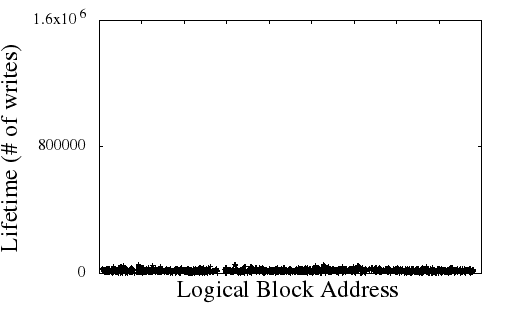
\includegraphics[width=0.21\textwidth]{figure/type_1}} % data from 4/03031953 
	\hspace{2pt}
	\subfloat[Logging (manual)]{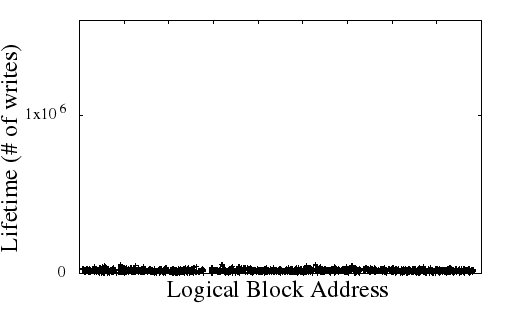
\includegraphics[width=0.21\textwidth]{figure/pcID_2}}
\hfill
\vspace{-1pt}
	\subfloat[Flushing (PC)] {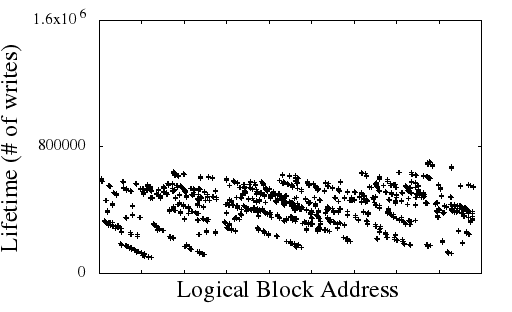
\includegraphics[width=0.21\textwidth]{figure/type_3}}
	\hspace{2pt}
	\subfloat[Flushing (manual)]{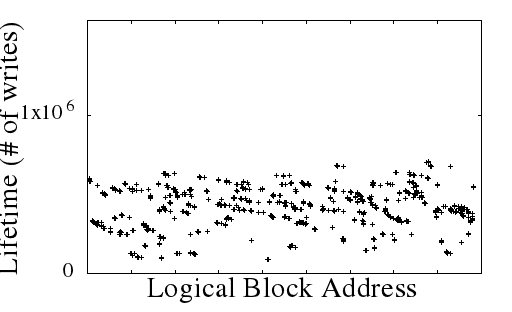
\includegraphics[width=0.21\textwidth]{figure/pcID_3}}
\vspace{-10pt}
\caption{Data lifetime distributions of different PCs.} 
\label{fig:types_and_PCs}
%\vspace{-15pt}
\end{figure}


In order to validate our hypothesis that PCs can be useful for predicting
lifetimes by distinguishing dominant I/O activities, we conducted experiments
using RocksDB, comparing the accuracy of identifying dominant I/O activities
using two different methods.  First, we manually identified dominant I/O
activities by inspecting the source code. Second, we automatically decided
dominant I/O activities by extracting PCs for write-related system functions.
Fig.~\ref{fig:types_and_PCs} illustrates two dominant I/O activities matched
between two methods.   As shown in Fig.~\ref{fig:types_and_PCs}(a)
and~\ref{fig:types_and_PCs}(b), the logging activity of RocksDB is correctly
identified by two methods.  Furthermore, from the logging-activity PC, we can
clearly observe that data written from the PC are short-lived. Similarly,
from Fig.~\ref{fig:types_and_PCs}(c) and~\ref{fig:types_and_PCs}(d), we observe
that data written from the flushing-activity PC behaves in a different fashion.
For example, data from the flushing-activity PC remain valid a lot longer than
those from the logging-activity PC.


